%%%%%%%%%%%%%%%%%%%%%%%%%%%%%%%%%%%%%%%%%%%%%%%%%%%%%%%%%%%%%%%%%%%%%%%%%%%%%%%%%%%%%%%%%%%%%%%%%%%%%%
%
%   Filename    : chapter_3.tex 
%
%   Description : This file will contain your Research Methodology.
%                 
%%%%%%%%%%%%%%%%%%%%%%%%%%%%%%%%%%%%%%%%%%%%%%%%%%%%%%%%%%%%%%%%%%%%%%%%%%%%%%%%%%%%%%%%%%%%%%%%%%%%%%

\chapter{Results and Analysis}
This chapter contains all the results from the research conducted and the corresponding analyses for the results.

\section{t-SNE Visualization Results}
After t-SNE was applied on the dataset as was discussed in Chapter 4, the resulting points were plotted according to different categories. For the entire set of t-SNE plots, please refer to Appendix F.

\subsection{Per Period Plot}
Figure 5.1 shows the plots for different musical periods. Each of the colors represent a different composer in each period:  blue for composer 1, green for composer 2, red for composer 3, purple for composer 4, and yellow for composer 5. All five periods had a similar shape of a ball since all of them represents an entire period of music and it would only be appropriate that the points are evenly scattered in the plane. Baroque period, however, has an obvious lack of plotted points in the figure compared to the others since this period in particular had the lowest number of data points originally due to the fact that the symphonies from here are generally shorter in time span. 20th Century, on the other hand, shows a more concentrated ball shape as opposed to others since this period had symphonies that are generally longer than that of other periods.

\begin{figure}[!htb]
\caption{Per Period Plot}
\centering
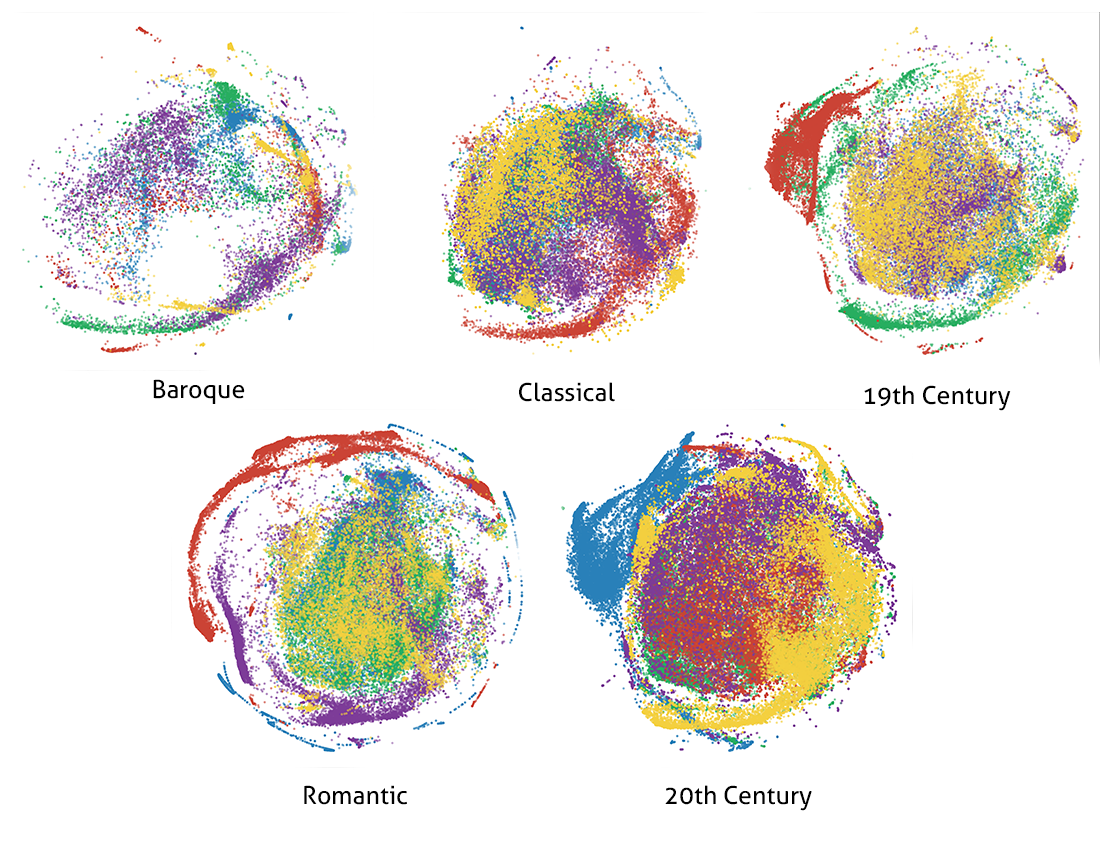
\includegraphics[scale=0.5]{per_era}
\end{figure}

\subsection{Per Composer Plot}
Figure 5.2 shows the plots of the different composer through each period. The first row of plots are from the Baroque Period, then plots from the Classical, 19th Century, Romantic and 20th Century Periods respectively.

\begin{figure}[!htb]
\caption{Per Composer Plot}
\centering
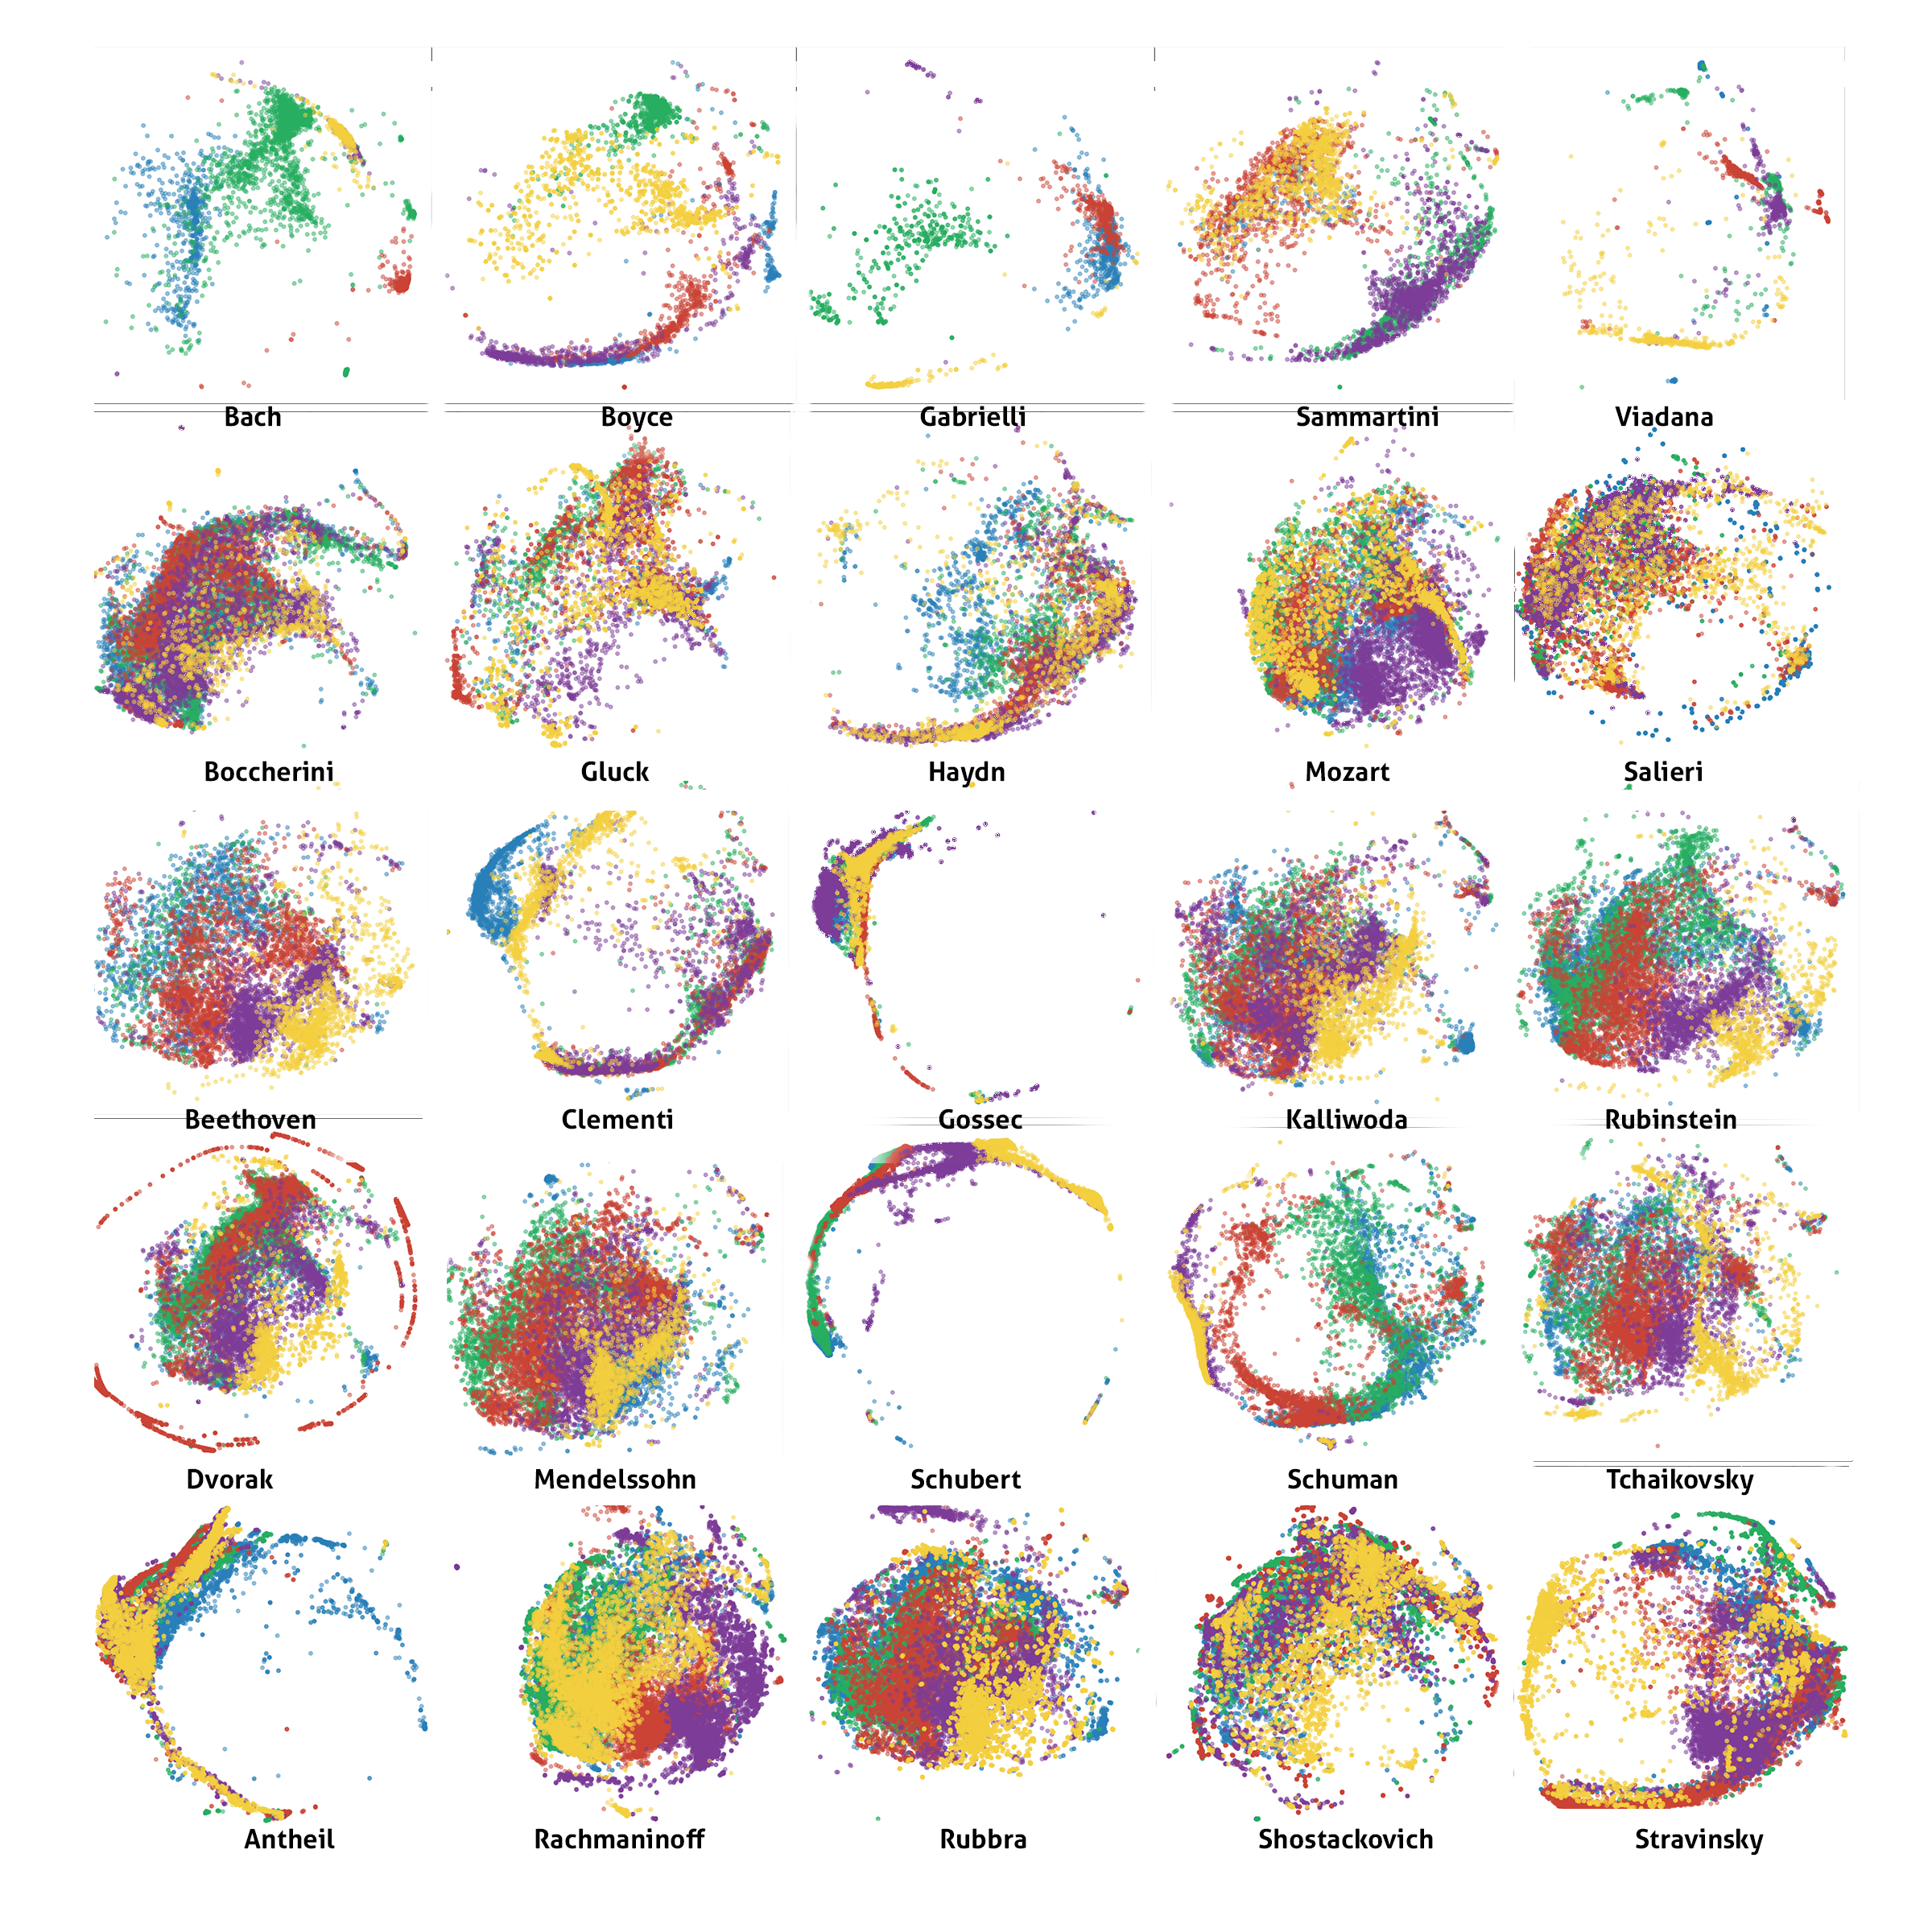
\includegraphics[scale=0.25]{per_composer}
\end{figure}

\subsection{Per Symphony Plot}
In order to represent the time-series aspect of the visualization, the researchers color graded the plotted points as the points aged. The colors span from yellow to green, to blue and to violet, from start to end respectively. An example of this gradation can be seen in Figure 5.3, which is the plot of (P5C2S5).

\begin{figure}[!htb]
\caption{Symphony Plot}
\centering
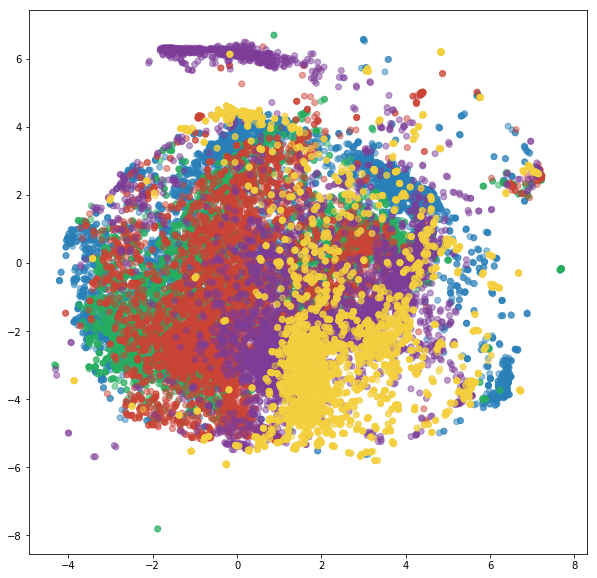
\includegraphics[scale=0.5]{P5C3}
\end{figure}

The gradation is done to all symphonies and is grouped and presented by music period. Figures 5.4 to 5.8 show the plots of each symphony as it progresses through time. 

\begin{figure}[h]
\caption{All Symphonies Part 1}
\centering
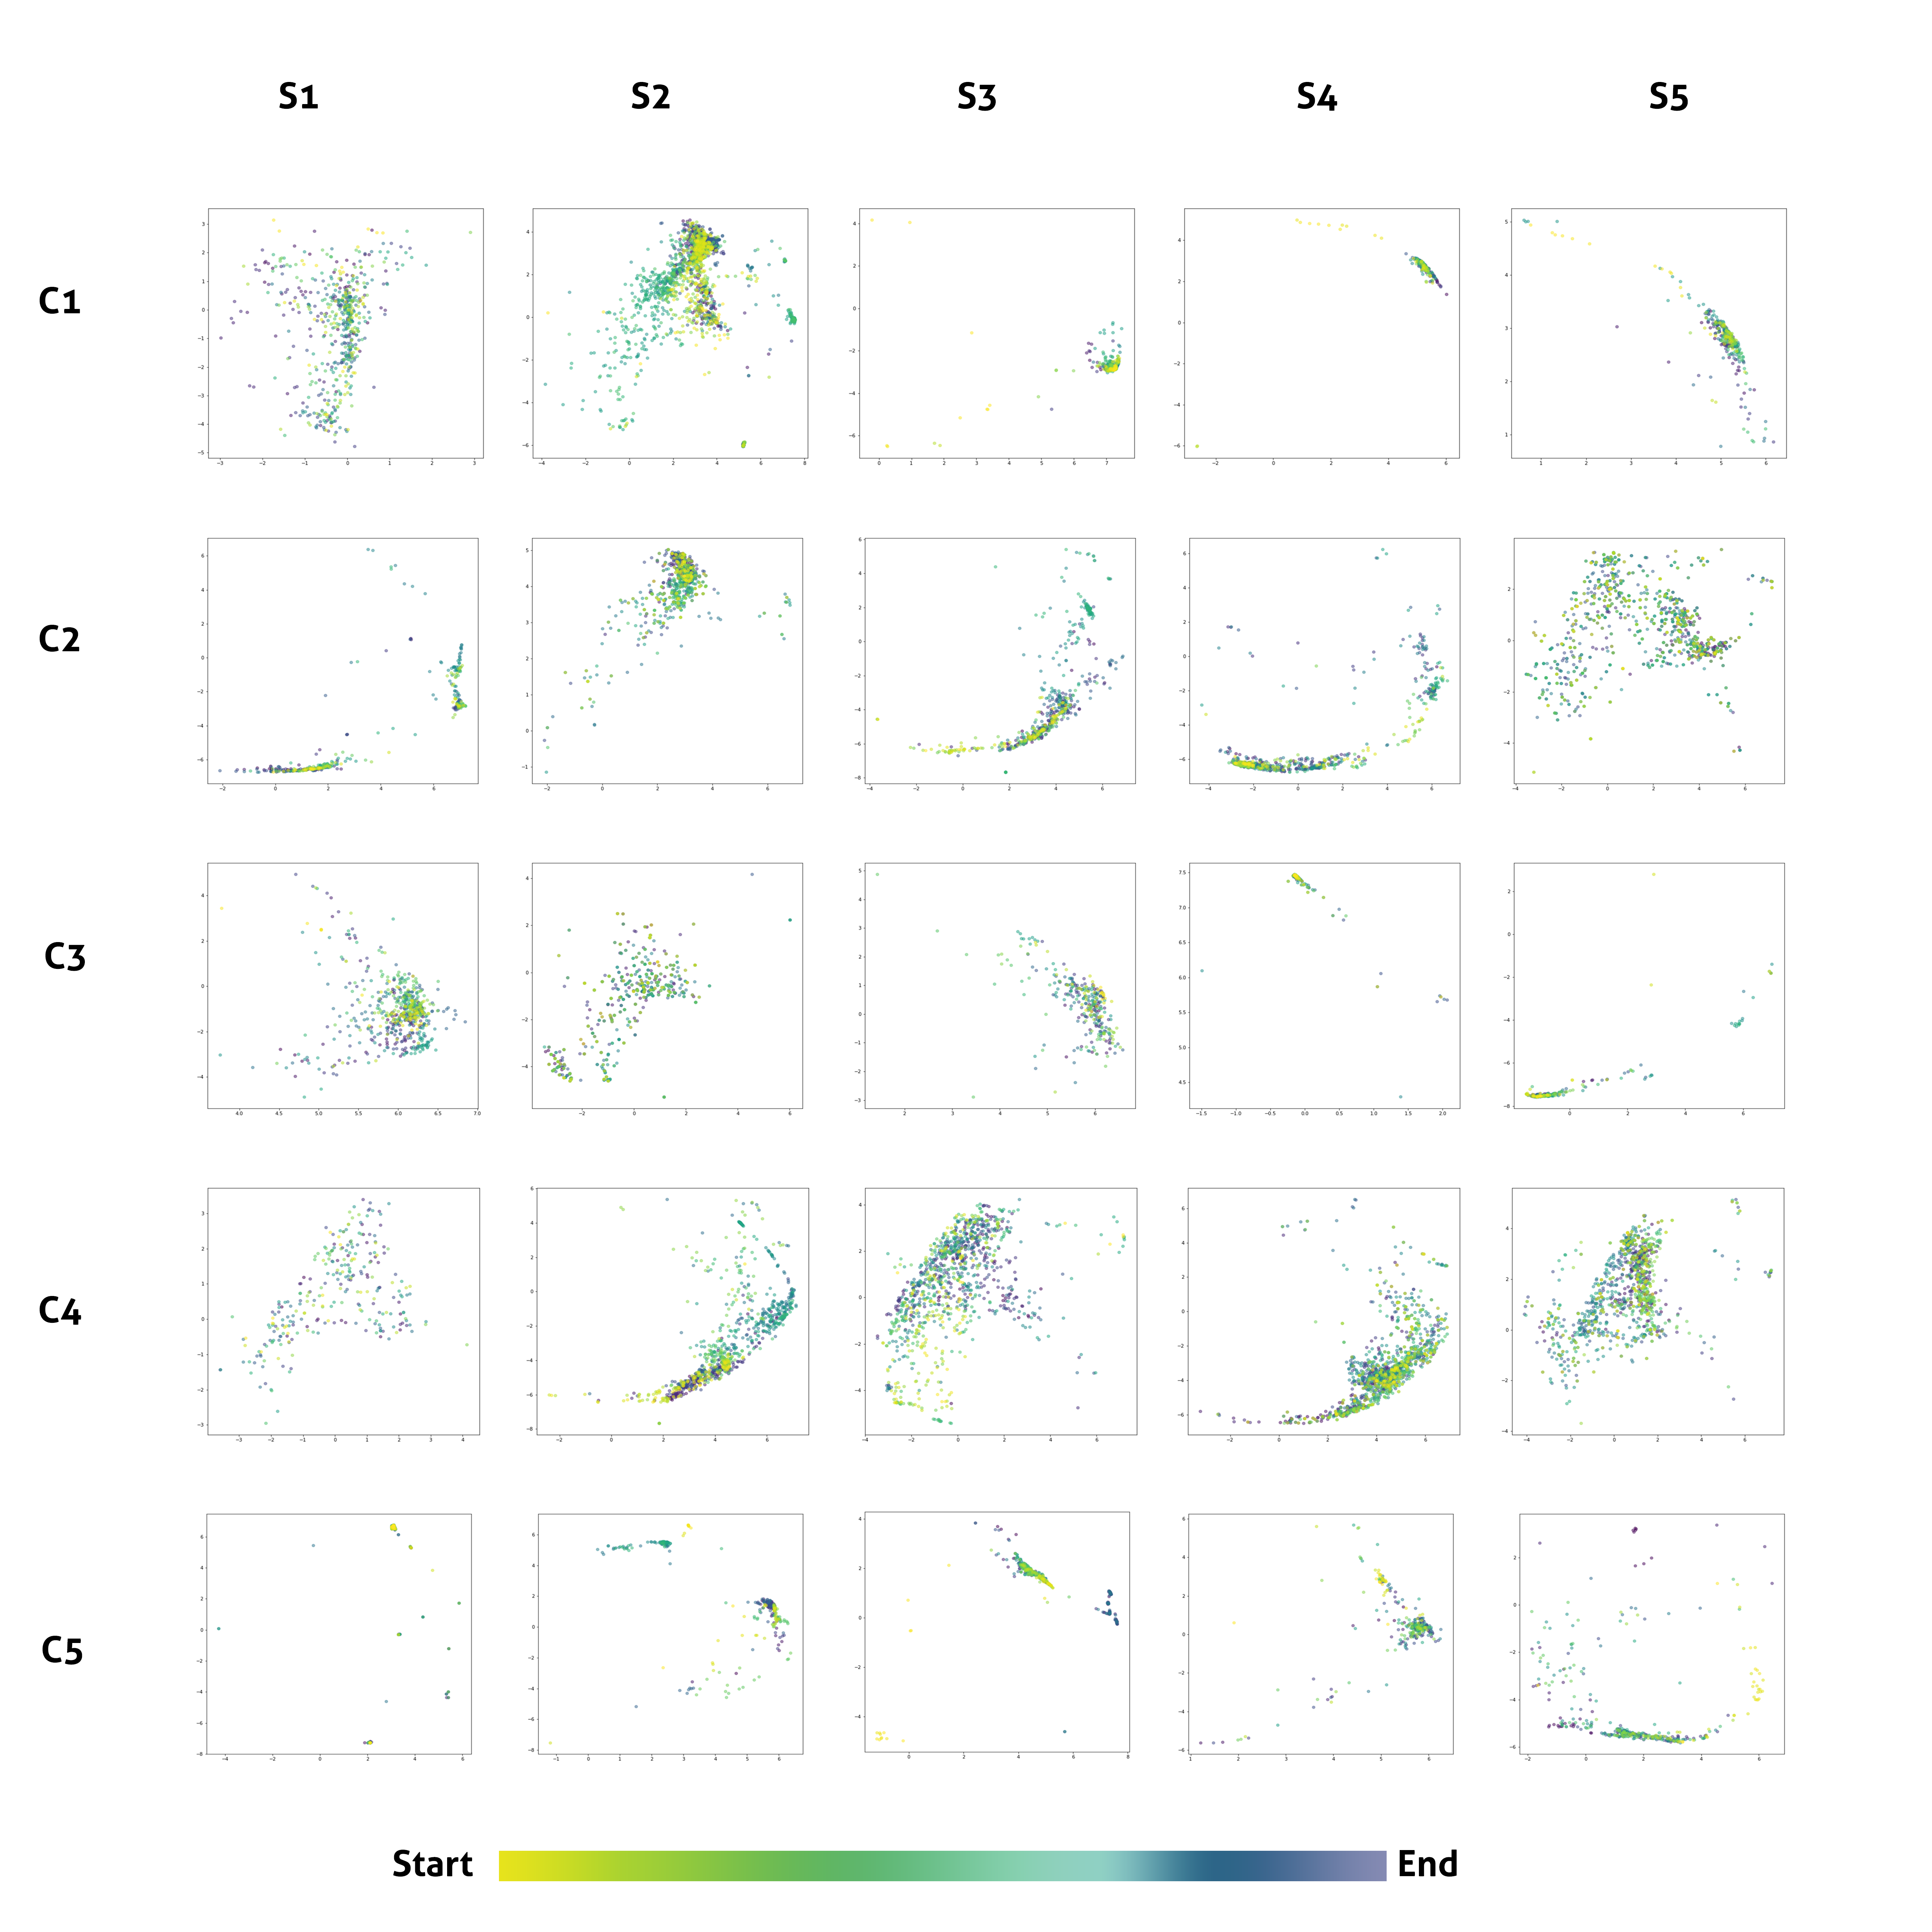
\includegraphics[scale=0.08]{p1-2_allsymphonies}
\end{figure}

\begin{figure}[h]
\caption{All Symphonies Part 2}
\centering
\includegraphics[scale=0.08]{p2_allsymphonies}
\end{figure}

\begin{figure}[h]
\caption{All Symphonies Part 3}
\centering
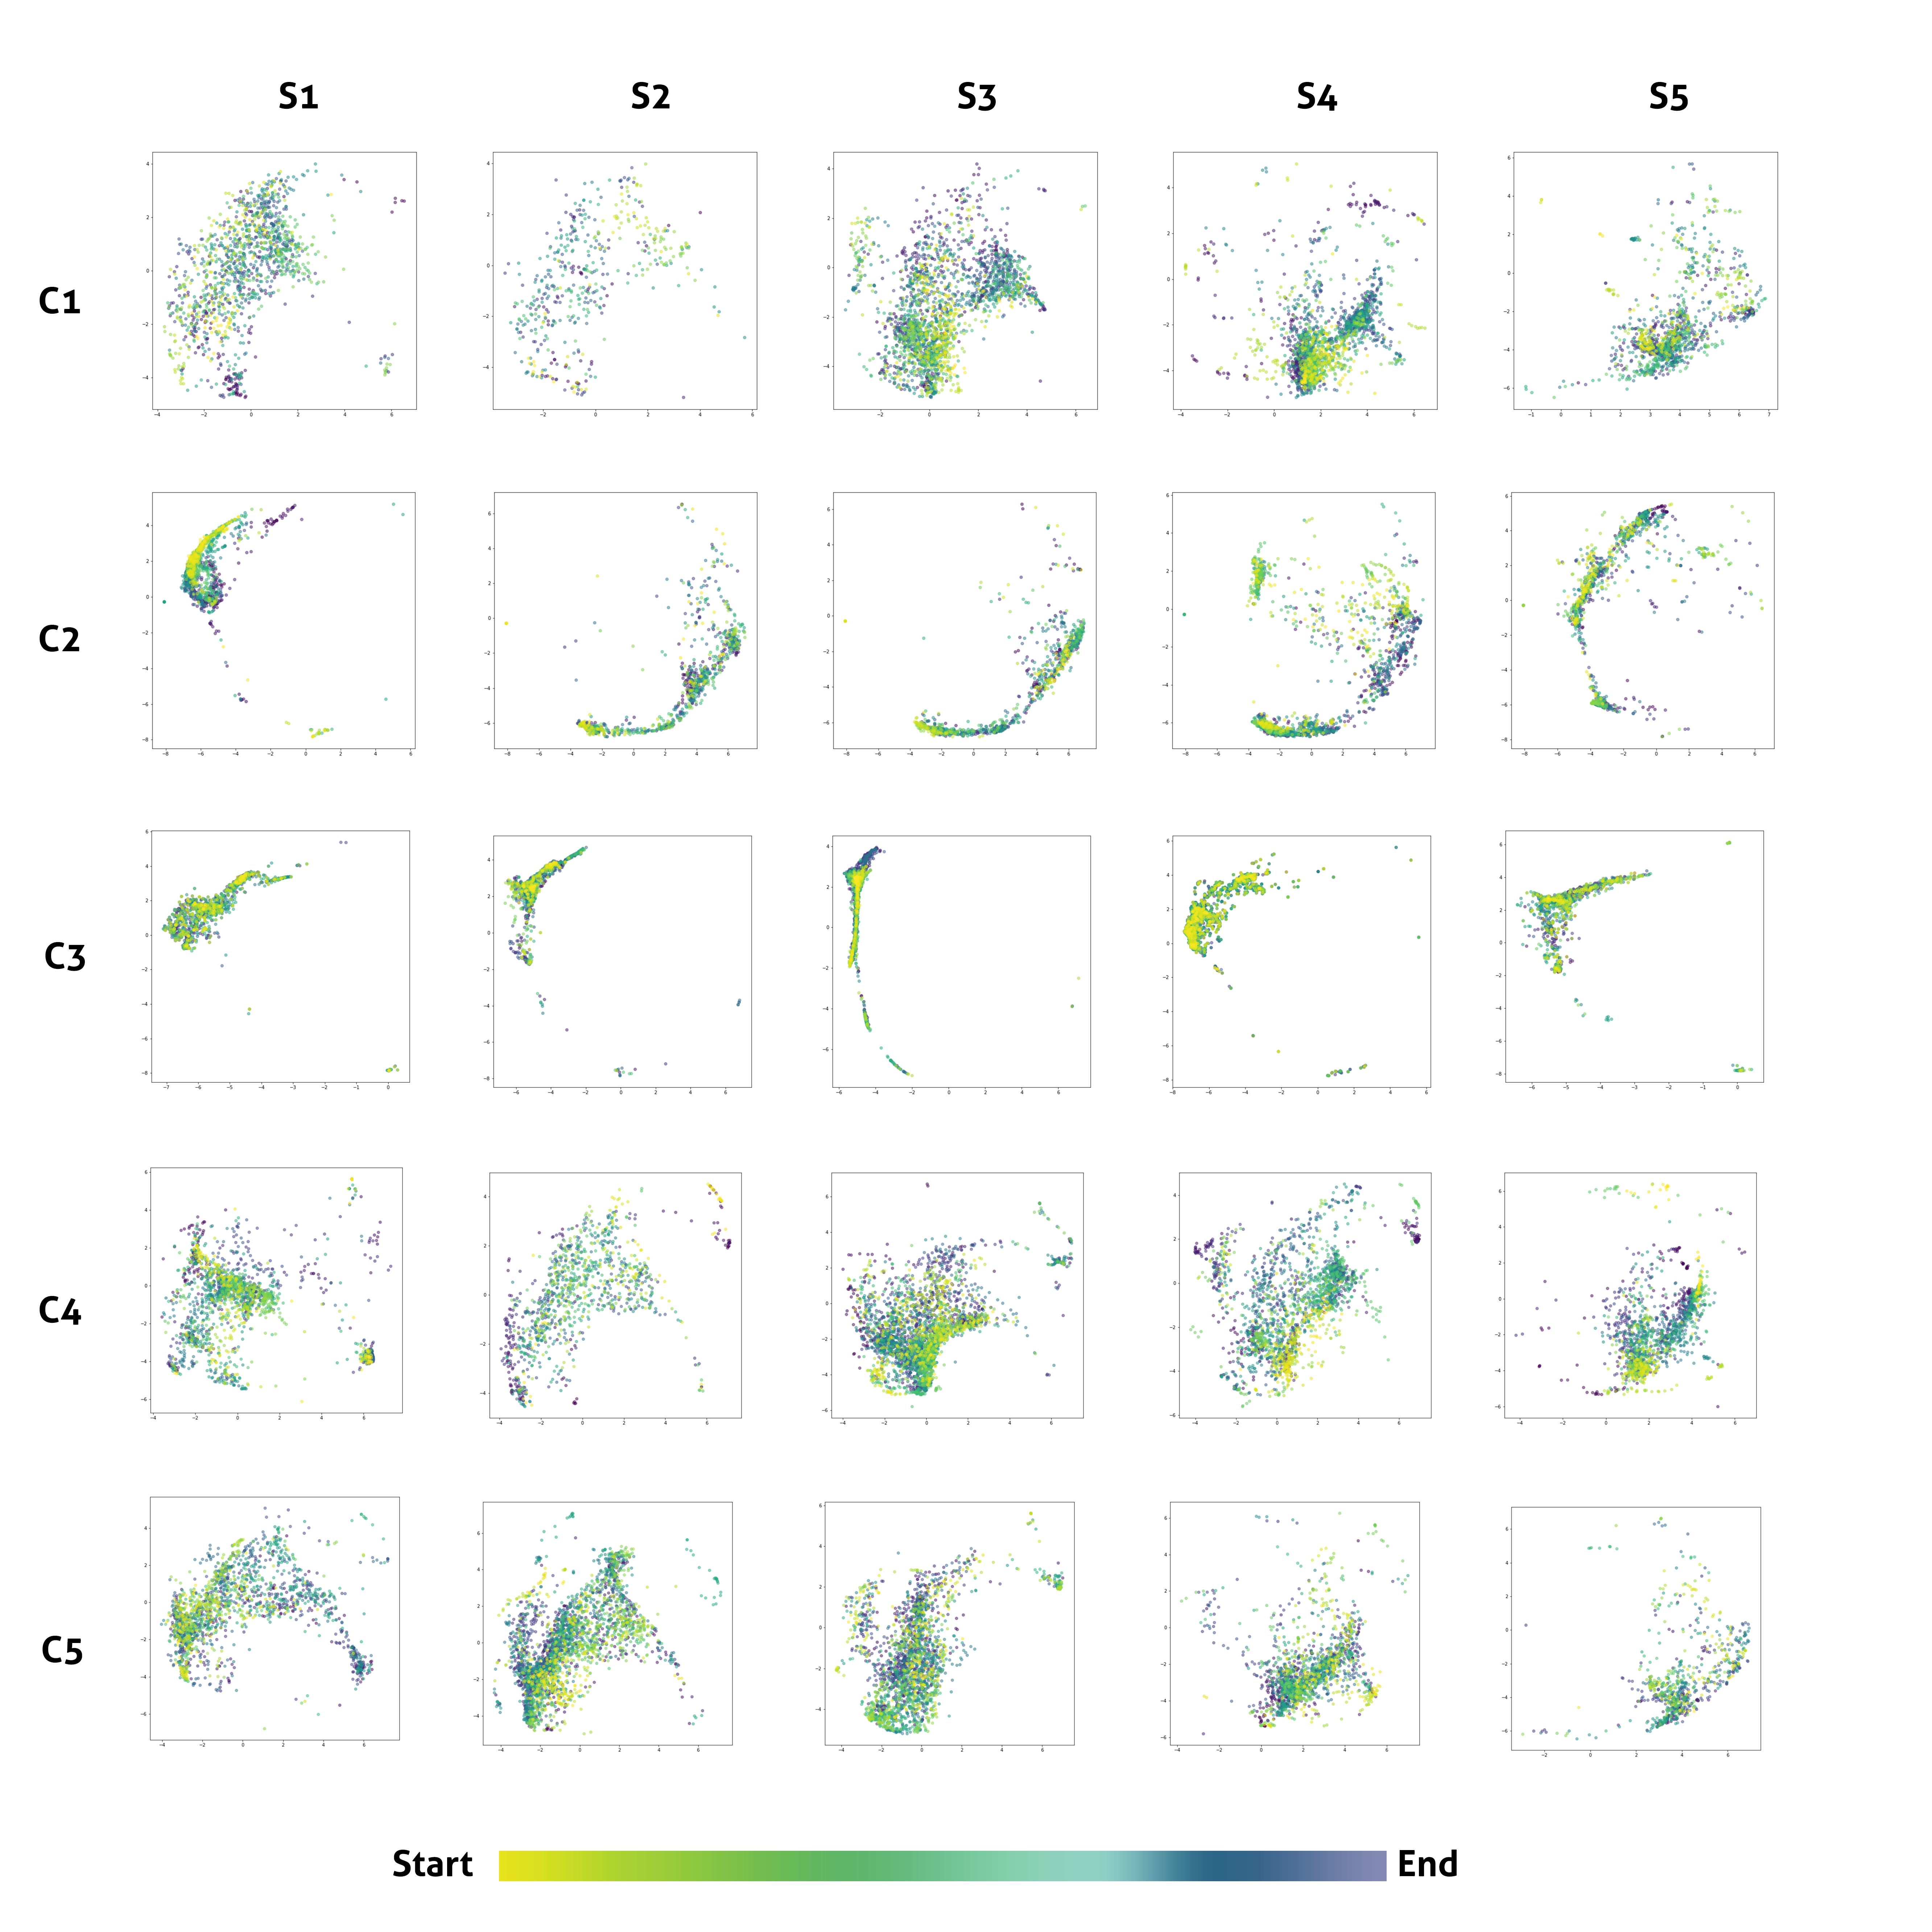
\includegraphics[scale=0.08]{p3_symphonies}
\end{figure}

\begin{figure}[h]
\caption{All Symphonies Part 4}
\centering
\includegraphics[scale=0.08]{p4_allsymphonies}
\end{figure}

\begin{figure}[h]
\caption{All Symphonies Part 5}
\centering
\includegraphics[scale=0.08]{p5_allsymphonies}
\end{figure}